% !TEX root = ../main.tex


\chapter{研究方案}

\section{研究目标、内容和拟解决的关键问题}
\section{拟采取的研究方法、技术路线、试验方案及可行性分析}
\section{研究的创新点}
\section{研究计划及预测进展}
\section{研究目标、内容和拟解决的关键问题}
\chapter{预期研究成果}

并行计算(Parallel Computing)一般是指许多指令得以同时进行的计算模式。在同时进行的前提下,可以将计算的过程分解成小部分,之后以并发方式来加以解决。

空间上的并行导致两类并行机的产生,按照麦克·弗莱因(Michael Flynn)的说法分为单指令流多数据流(SIMD)和多指令流多数据流(MIMD),而常用的串行机也称为单指令流单数据流(SISD)。MIMD类的机器又可分为常见的五类:并行向量处理机(PVP)、对称多处理机(SMP)、大规模并行处理机(MPP)、工作站机群(COW)、分布式共享存储处理机(DSM)。

% 首先介绍CPU下的并行方案OpenMP,这是一种基于共享内存的多线程程序库,采用Fork-Join模型来对程序中的循环部分进行并行化,程序员可以实现增量式开发,不再需要花费大量的精力在线程的创建、同步与销毁上。使用OpenMP开发的程序具有良好的可移植性和扩展性。

% 其次,针对CPU运算能力不足的问题,引出了CPU-GPU协同计算模式,充分发挥GPU并行处理数据的能力,将CPU从繁重的计算任务中解放出来,着重负责逻辑的控制和数据的存取,合理地将部分程序并行执行,从而达到提升效率的目的。

% 再次,详细介绍了两个面向CPU-GPU协同计算的并行框架,CUDA和OpenCL。两个框架的模型基本类似,但是CUDA是针对Nvidia显卡做的设计,更贴近底层硬件,可以根据硬件特点设计出几十上百倍的效率优化;OpenCL的设计兼容性则很强,模型设计兼容各大硬件厂商的CPU、GPU、DSP,虽然牺牲了部分根据硬件特点可能做出的优化,但大大提高了应用程序的可移植性。两者各有优势,在不同的环境下可以发挥不同的特长。

\section{OpenMP}
OpenMP是一种基于共享内存实现的并行程序设计库,它的并行依靠多线程来实现,特别适合在多核CPU上进行并行程序开发设计。是用户对共享主存编程模型最新要求的全面反映。现今大多数编译器,例如Sun Compiler、GNU Compiler、Intel Compiler、Visual Studio等等,都已经支持了OpenMP。程序员可以使用C、C++、Fortran等众多流行的编程语言来实现OpenMP并行程序。在程序设计时,编程人员只需要在需要并行执行的代码段前加入适当的OpenMP预编译指令,在必要的时候加入一些线程通讯指令,编译器就会根据自身情况(是否支持OpenMP)自动将代码并行化。这种简单的编程模式,使得程序员可以将更多的精力放在算法本身,不用过多考虑并行线程的设计细节。
\begin{figure}[htbp]
	\centering
	\includegraphics[width = 0.5\linewidth]{forkjoin.png}
	\caption{Fork-Join并行模式}\label{fig:forkjoin}
\end{figure}
OpenMP的并行模式是Fork-Join模式,程序开始时只有一个主线程,再碰到需要并行的任务时,执行Fork操作,派生出多个线程共同完成任务,当这个任务完成时,各个线程进行Join操作,回到一个主线程继续串行执行下面的操作,如\autoref{fig:forkjoin}所示。通过这种模式,程序员可以在设计时方便地添加各种并行模块,采用增量式的方式进行开发。由于各个模块在执行时是独立的,所以在性能调试时,只需要考虑单个并行模块的调整。在设计OpenMP程序时,主要考虑的问题是循环的并行化处理,通常情况下Fork-Join的边界就是循环的边界,即在循环开始的时候生成大量线程,并行执行循环内部的代码,当循环结束的时候销毁这些并行线程,回归串行的主线程。所以如何消除变量数据在循环中的依赖性,如何设计循环的层次结构成为设计高效的并行OpenMP程序的关键。

\subsection{OpenMP编程模式}
OpenMP是为在多核处理器上编写并行程序而设计的一个应用编程接口,它包括一套编译指导语句、一个用来支持它的函数库和一些环境变量。编译指导语句中规定了程序并行化的一些参数和细节,编译器会根据这条语句自动将程序编译成并行的代码,通常由指令和子句列表两部分构成。函数库主要包括执行环境函数、原子操作函数、时间操作函数等,根据这些函数可方便和灵活地操作和控制程序运行时的线程、变量,实现了串行程序并行化的过程。环境变量用来控制并行执行的方式,例如OMP\_DYNAMIC表示是否允许改变线程数量,OMP\_NUM\_THREADS设置了默认的线程个数。

在OpenMP中,线程之间通过共享内存进行数据通讯,不同的处理器共享同一块内存,这就是OpenMP的共享存储模型。OpenMP的变量分为私有变量和公有变量两种类型。私有变量是各个线程自己创建并维护的数据副本,相互之间不会产生任何影响;公有变量则存储在共享内存中,是对原始数据的直接引用,当存在多个线程对其进行操作时,需要进行原子性控制来避免数据竞争带来的错误。所以如何设计数据的存储形式是保障并行OpenMP程序准确运行的关键问题。

有两种常用的方式来开发OpenMP并行程序。一种是采用Fork-Join模型将程序中的循环部分(即计算密集的部分)进行并行化,这是一种简单的循环级并行。第二种是SPMD(Single Program Multi-Data,单程序多数据)模式,需要程序员对代码中的计算部分进行详细分割,根据计算的逻辑特点和密集程度合理地进行任务分配和内存分配。Fork-Join模式的优势在于程序实现起来简单便捷,可以实现增量式的开发;SPMD的优势则在于可以更有效地利用计算资源,程序的运行效率也更高。对于一般的应用程序,程序员们更倾向于选择Fork-Join这种简洁的开发模式。

\subsection{OpenMP的特点与应用}
从上面的简单介绍中,可以总结出OpenMP具有以下特点:
\begin{enumerate}
\item	良好的可移植性:OpenMP被众多主流编程语言、编译器、操作系统所支持,基于OpenMP开发的并行程序可以轻易地移植到各种应用环境中。
\item	易实现:OpenMP并行程序的开发实现方式简单,Fork-Join模式使得程序可以进行增量式开发,并行模块的边界就是循环模块的边界,各个并行模块之间相互独立,程序员不再需要花费大量的精力在线程的创建、同步与销毁上,也不需要考虑计算负载的平衡,这不仅减小了程序的设计难度,程序的调试优化难度也大大降低了。
\end{enumerate}
随着电子数据爆炸式地增长,OpenMP在很多领域得到了应用,包括机械工程、医学、物理学、天文学、管理科学等等。

% \section{CPU-GPU协同计算}
% 随着计算机硬件的发展,拥有着更多计算核心的GPU逐渐承担起密集的计算任务,基于GPU的算法设计越来越流行。然而就算是一个简单的算法,仅仅依靠大量的并行计算也是不够的,还需要复杂的逻辑控制,控制数据的存取,控制循环计算的次数等等,这些任务则需要擅长逻辑控制的CPU来完成。因此,一个高效、精确的算法设计通常需要CPU-GPU协同计算。下面我们就介绍CPU与GPU的性能对比,以及协同计算的设计理念。
% \subsection{CPU与GPU性能对比}
% CPU主要负责解析计算机指令、执行指令操作、控制时间、处理数据等功能,是一台计算机的控制核心。在过去的40多年中,凭借缓存策略的优化、超流水线、超标量、多核技术的发展,CPU的性能得到了极大地飞跃[56]。但是近几年来,CPU的发展似乎遇到了瓶颈,这个瓶颈不仅仅来自半导体工艺的限制,还因为CPU的内部电路十分复杂,使其不能像GPU那样依靠堆积计算核心数量来提升性能,在CPU中每增加一部分电路都需要经过很长时间的设计和研发。此外,CPU需要处理的指令往往是互相关联的,例如分支、循环、迭代等等,为了准确执行这些关联的指令,CPU不得不采用顺序执行的设计,这就使得计算性能很难提高。随着IT行业的不断发展,各个行业每天都在产生大量的数据,在这种情况下,CPU的计算负担越来越大,迫切需要计算机主板上的其它芯片来分摊计算压力。此时,具有众多计算核心的GPU就成为了一个很好的选择。
% GPU是专为复杂的数学计算和几何运算设计的,主要负责图形的渲染工作。近些年市场对高清、三维图形的处理的需求不断提高,尤其是游戏产业对图形的实时处理要求的提升,推动了图形处理器(GPU)的不断进步,GPU已经演化成能够提供多线程计算并拥有并行处理能力的处理器,大量数据元素被映射到并行处理的线程上进行处理。这种并行加速的应用,也从单纯的图形处理领域渐渐扩展到信号处理、建模仿真、金融预测、生物计算等等大数据处理领域。
% CPU与GPU在数据处理、命令执行的方面各有特长,下面对比了两者之间的不同。
% \begin{enumerate}
% \item	硬件架构:根据不同的设计目标,CPU和GPU通常应用在不同的场景下。CPU的计算任务中通常包含各种不同的数据类型,这就需要CPU在设计时具有很强的通用性,此外逻辑判断指令又会带来大量的分支、跳转和中断等处理。相对而言,GPU则面对的是类型较为统一的、相互依赖性低的、规模较大的数据,以及没有分支、中断的单一计算环境。这就导致CPU和GPU在硬件架构上呈现出很大的不同。如\autoref{fig:cpu_vs_gpu}所示。图中绿色的部分是计算单元,黄的是控制单元,橙色的是存储单元。从图中我们可以看出,在GPU中存在大量的计算单元,存储和控制单元被大大简化。而CPU中,大量的空间被存储单元,而且还有复杂逻辑控制单元和图中没有展示的诸多优化电路,相比之下计算单元在CPU中只占了一小部分。所以,GPU擅长的是大规模并发计算,CPU则更擅长逻辑控制。
% \begin{figure}[htbp]
% 	\centering
% 	\includegraphics[width = 0.5\linewidth]{cpu_vs_gpu.png}
% 	\caption{CPU与GPU的硬件架构对比}\label{fig:cpu_vs_gpu}
% \end{figure}
% \item	存储带宽与缓存模式:在存储带宽方面,GPU相比CPU具有较大优势,举个例子,GT200的显存带宽是140GB/s,是同时期的CPU内存带宽的5倍。在缓存方面,CPU需要耗费大量的资源进行复杂的逻辑控制,来保证数据在缓存和内存的一致性。在多线程运行环境下,一旦切换线程的上下文,就需要重建一次缓存上下文,每次重建都会耗时几十到上百个时钟周期。在GPU中,缓存则是只读的,省去了复杂的逻辑控制,缓存的主要作用是过滤对显存的访问指令,以减少对显存的直接访问,节约显存带宽。综上,GPU的计算单元访问存储器或是缓存的速度都较CPU更快。
% \item	核心数量:通常情况下一个CPU只具有2-8个核心,虽然超线程技术可以将一个核心虚拟成多个核心,但是在同一个时刻每个虚拟核心也只能执行一个线程。GPU则包含成百上千个计算核心,进行细粒度的并行计算。
% \item	线程:通常情况下,在同一个时刻每个CPU核心只能执行一个线程,也就是说CPU的多线程是一种粗粒度的多线程,依赖操作系统提供的应用程序接口来实现,当线程切换时,需要保存当前线程的上下文并装载新线程的上下文,每次上下文的切换都会造成几十到上百个时钟周期的损失。在GPU中,线程是轻量级的,零开销线程切换,多线程并发执行时这种灵活地切换机制可以有效地利用计算来隐藏资源等待带来的延迟。所以当计算任务和数据读写任务被合理分配时,就可以大幅度隐藏线程切换带来的延迟。
% \item	计算能力:通过上述的分析,我们可以发现相比于CPU,GPU更专注于数据处理,它大大减少了逻辑控制单元和缓存,将大量硬件资源投入计算单元,这使得GPU的单精度浮点数处理能力远远超过了同时代的CPU产品,见\autoref{fig:flops-per-cycle-dp}。虽然近些年多核CPU层出不穷,但受到工艺、材料等物理上的限制,数据计算能力很难有突破性的飞跃,因此GPU在大数据处理中将发挥越来越重要的作用。

% \end{enumerate}
% \begin{figure}[htbp]
% 	\centering
% 	\includegraphics[width = 0.5\linewidth]{flops-per-cycle-dp.png}
% 	\caption{GPU与CPU单精度浮点数运算能力对比}\label{fig:flops-per-cycle-dp}
% \end{figure}
% 通过上述对比,GPU虽然表现出了强大的计算能力,但是却有无法处理分支、迭代等复杂逻辑的短板,使其无法独自完成实际应用的需求,这就需要擅长处理复杂逻辑的CPU来配合。CPU-GPU协同计算就是利用两者各自的优势,充分发挥GPU的计算能力,CPU则着重负责程序的逻辑控制和数据读写,从而提高程序的运行效率。
% \subsection{CPU-GPU协同计算设计理念}
% CPU-GPU协同计算就是充分发挥两者各自的优势,合理地将部分程序并行执行,从而达到提升效率的目的。相比于传统的并行加速方式,CPU-GPU协同计算具有一定的优势。“天河一号”就是釆用了这种协同计算模式来获得超强的计算能力,共包含7168组CPU与GPU协同的计算节点,每个节点由2个CPU与1个GPU组成。
% 通过上一节的性能对比可以看出, CPU采用了复杂的控制逻辑和分支预测,使线程能够迅速地获得指令和数据,大量的缓存被用来提高个别线程的效率,对延迟极为敏感;而 GPU 则是通过大量功能简单的流处理器共同运转来提高计算和数据的整体吞吐量。相比于仅使用多核CPU来实现的并行加速,CPU-GPU协同计算更有优势。
% 分布式计算通过网络将计算节点组织起来,使各个节点可以协作完成计算任务。数据的传输和指令的发布都需要通过网络,在程序设计时需要着重考虑数据在网络中的传输方式,避免产生通信拥塞。CPU-GPU协同计算中的数据传输主要集中在CPU内存和GPU全局内存之间,通过PCI-E接口完成,相比于分布式计算,数据的传送要方便、快捷很多。
% 此外,CPU-GPU协同计算还有具有性价比高的优势,主流GPU的运算能力可以达到同期主流CPU的10倍左右,但价格只有2-3倍。CPU-GPU协同计算可以在单机环境下实现,这使得每个人都能以较小的代价获得超级计算能力。没有了外界环境的限制,单机CPU-GPU协同计算应用的范围也更加灵活。
% 随着CPU-GPU协同计算越来越热门,为了增强GPU的可编程性,研究人员提出了许多新技术,使得针对GPU的并行程序开发变得更加简便,下面两节我们将详细介绍CUDA、OpenCL这两种并行编程框架。


\section{CUDA计算平台}
从上一节的介绍中,我们知道了GPU具有强大的计算能力。最初,程序员通过图形绘制接口OpenGL、DirectX,来进行图形领域的程序设计。在程序设计过程中,程序中的算法不得不被表达成图形流水线的概念,才能被GPU高效执行,这大大增加了程序开发难度,使得这类GPU语言下的通用计算的使用范围被限制于高端图形设计人员中。为了使GPU强大的计算能力更加通用化,不再限制于图形领域,斯坦福大学图形实验室设计开发了BrooK语言,该语言使得开发人员不再需要了解图形流水线,只需要根据功能需求设计读写函数和并行计算的核函数,这大大降低了GPU通用计算的门槛。随着专门为通用计算设计的统一渲染架构渐渐代替原来的图形流水线架构,原来的GPU通用计算框架也渐渐被淘汰,GPU的通用计算也进入了全新的层次,NVIDIA提出的CUDA计算平台开始在GPU通用计算领域扮演越来越重要的角色,下面我们将详细介绍CUDA计算平台。
\subsection{CUDA简介}
为了适应CPU-GPU协同计算的需求,NVIDIA公司于2006年推出了CUDA,作为GPU通用计算的并行计算平台和编程模型。程序员不再需要使用复杂的图形接口OpenGL、DirectX等进行GPU编程,以方便地使用C语言开发基于GPU的并行程序。这大大降低了GPU通用计算的开发难度,使得大部分数据并行程序可以通过简单的算法修改得到性能上的大幅提升。CUDA为程序开发人员提供了便捷的GPU通用计算平台,一经推出就被广泛使用。
目前,CUDA仅被NVIDIA 自己研发的新架构GPU支持。但是这些 GPU 几乎涉及到了NVIDIA 公司在各个领域的产品,GeForce GTX 1080,GeForce GTX 980M等用于普通电脑的GeForce系列、Tesla C1060、Tesla S1070等面向通用计算领域的Tesla系列,Quadro M6000、Quadro K1200等针对图像处理领域的Quadro系列。但是这些GPU在图像处理、音频处理、金融预测、物理仿真、分子模拟、生物计算、石油勘测等领域,发挥着不可替代的作用。换言之CUDA并行计算平台已在众多领域中广泛应用。
% \subsection{CUDA硬件架构}
% 近10年来,随着大数据处理的需求越来越高,GPU的硬件体系架构也在不断更新,先后出现了Tesla、Fermi、Kepler、Maxwell、Pascal5种硬件架构。分析表格中的数据,总的发展趋势是处理器越来越多、内存越来越大、访问带宽越来越宽,总的来说就是显卡的并行能力越来越强、数据处理速度越来越快。下面我们就拿比较常用的Kepler架构来解释GPU各个部分工作原理,其它的架构均是类似。

% 展示了Kepler硬件架构,图中展示了一个SM(Stream Multiprocessor,流多处理器)中的所有结构,图中每个core都代表一个计算核心,每个核完全由浮点和整数算术逻辑单元组成,这也是真正执行计算的部分,此外还有32 个特殊功能单元 (SFU) 和 32 个加载/存储单元 (LD/ST)。每个SM中都有64KB的缓存空间供所有core访问。SM以32个并行线程为一组的形式调度进程,这32个并行线程叫做 Warp。图中可以看到,每个 SM中拥有四组Warp Scheduler和八组Instruction Dispatch单元,所以Kepler允许四个Warp同时发出执行,可以指派2个独立的指令给每个Warp。所有指令在硬件中以warp 为单位执行。所以这种每次循环中可以执行4个warp、8个指令的硬件结构(Tesla架构中每个SM中只包含8个核心,每个wrap指令则需要执行4个循环),可以大幅提高程序在硬件层面上的执行速度。

% \begin{figure}[htbp]
% 	\centering
% 	\includegraphics[width = 0.5\linewidth]{keplerSM.png}
% 	\caption{kepler硬件架构}\label{fig:keplerSM}
% \end{figure}

\subsection{CUDA存储模型}
GPU 的存储器层次结构相比于CPU更加复杂,在CUDA中存在多种不同的存储空间,不同的存储空间在访问带宽和容量等方面有很大不同,这也给程序员提供了更多的存储数据的方式。\autoref{fig:keplerSM}展示了CUDA的存储模型。包括了4个可读写内存:全局内存(Global Memory)、局部内存(Local Memory)、共享内存(Shared Memory)、寄存器(Registers),以及两个只读内存:常量内存和纹理内存。
全局内存位于显存上,是容量最大的一类存储空间,所有线程都可以访问全局内存,由于访问距离较远和缺少缓存的原因,这也是访问速度最慢的一块存储空间。常数内存也位于显存上,只能读取,通常比较小,只有64K,存储一些需要频繁访问的变量,由于具有缓存空间,所以这块空间的访问速度较快。类似的纹理内存也是一块位于显存上的只读空间,由原本用于纹理渲染的的图形专用单元发展而来,具有缓存加速,支持一维、二维、三维的纹理,空间要比常量内存大得多,适合用于图像处理或查找表,对数据量较大时的随机数据访问有良好的加速效果。寄存器是GPU芯片内的高速缓存,每个线程都有属于自己的寄存器,存储程序中需要使用的变量,访问速度是最快的,但是每个SM中寄存器的数量是有限的,程序运行时被SM内的所有线程均分使用。共享内存也在GPU芯片内,具有和寄存器相当的访问速度,同样大小有限,通常只有64K,可以被同一组线程共同访问,在使用时可以利用这一特性加快数据读写速度,但是也要注意多线程同时访问的过程中,产生的数据是否需要原子操作的问题。局部内存是全局内存中开辟出来的一块空间,访问速度也是比较慢的,它是寄存器的备用空间,当有过多的变量被声明时,寄存器存储不下的变量将会被放入局部内存中,这块空间也是每个线程独占的,其它线程无法访问。所以在程序设计时需要严格控制并行程序中的变量数量,过多的变量会被存在具备内存中,对这些变量的频繁访问会极大拖慢程序的运行速度。
\begin{figure}[htbp]
	\centering
	\includegraphics[width = 0.5\linewidth]{cuda_memory.png}
	\caption{CUDA存储模型}\label{fig:cuda_memory}
\end{figure}

\subsection{CUDA编程模型}
CUDA编程模型需要CPU-GPU协同计算,CPU作为主机负责程序的逻辑控制以及一些需要串行运行的部分,GPU则作为计算设备负责数据密集的并行计算任务。因此,一个完整的CUDA程序包括两个部分,由CPU串行执行的主机程序和由GPU并行执行的核函数(kernel)。主机程序主要负责准备数据、初始化参数、数据传输、循环控制、数据后处理等串行代码,并启动核函数。核函数负责大量数据的并行计算,由于GPU对于逻辑控制的不足,核函数中的分支、循环等操作会在并行执行的过程中带来大量线程等待,延长执行时间,所以在核函数中尽量执行简单的计算命令。在CPU上执行的主机程序,就如一般程序一样串行执行,下面我们来介绍核函数是如何在GPU硬件上并行执行的。
核函数中的计算任务在执行时被映射为大量可以并行执行的线程,并由硬件动态调度并执行这些线程。这些线程的组织形式如\autoref{fig:cuda_programming}所示,所有的线程被映射成若干个Grid,每个Grid由若干个Block构成,每个Block中又包含若干个Thread。实际的计算指令由Thread完成,同一个Block中的所有Threads是并行执行的,在这个Block中它们有唯一的threadIdx标识,在程序设计的时候可以根据这些标识区分不同的线程,控制不同的线程对不同的数据进行操作,即实现单指令多数据操作SIMD(Single Instruction Multiple Data)。此外,如\autoref{fig:keplerSM}所示每个Block中都有一块可以高速访问的共享内存,同一Block中的所有Threads可以利用这块共享内存相互通信。再向上看一个层面,每个Block在硬件上也是并行执行的,可以有属于不同Grid的Block并行执行,但是Block之间无法进行通信,Block之间也没有执行顺序。综上所述,CUDA的线程按照两个层次进行组织调度,一个是Block之间不需要通信的粗粒度并行,另一个是同一个Block中Thread之间允许通信的细粒度并行。这种双层的设计结构,使得核函数可以灵活地运行在不同硬件架构的GPU上,不管是较早的Tesla架构,还是最新的Pascal架构,每个Thread都会在硬件架构中的core当中执行,由于在硬件执行过程中是以32个线程为一组Wrap,所以在设计Block大小(即每个Block包含的Thread数量)时,不仅要考虑功能业务需求,还需要根据不同硬件架构下SM的结构,合理地做出设计,尽量避线程拥塞、等待。
\begin{figure}[htbp]
	\centering
	\includegraphics[width = 0.5\linewidth]{cuda_programming.png}
	\caption{CUDA线程组织方式}\label{fig:cuda_programming}
\end{figure}


\subsection{CUDA的特点与应用}
通过分析CUDA的架构,可以看出CUDA的在CPU-GPU协同计算方面有十分明显的优势,总结如下:
\begin{enumerate}
\item	编程模型:一个完整的CUDA程序被分为在CPU上执行的主机程序以及在GPU上执行的核函数,这种分离式的编码可以使得程序更加清晰,也使得CPU、GPU在程序执行时的分工更加明确,CPU负责复杂的逻辑控制,GPU负责简单的并行计算。此外在核函数并行执行时的线程组织结构,采取两个层次进行组织,这种设计不仅贴合GPU硬件的实际结构,分层次的管理也使得并行程序的设计更加灵活。
\item	存储结构:CUDA存储模型中多种不同访问带宽和容量大小的存储器类型,给程序的设计开发带来了极大的灵活性,程序员可以通过合理分配数据读写和计算任务,来隐藏线程切换带来的延时,提高总体的程序运行效率。
\item	编程语言:C语言是使用范围最广的一类编程语言,在此基础上扩展得到的CUDA C很容易被广大开发人员所接受,CUDA并行程序的开发难度也被大大降低。随着CUDA的日益流行,很多流行的编程语言都提供了CUDA的绑定,例如Python绑定为PyCUDA;Java绑定为JCuda;.NET绑定为CUDA.NET,GPU.NET;MATLAB绑定为MATLAB phag-in for CUDA;Fortran绑定为FORTRAN CUDA等。
CUDA为程序员提供了一个高效便捷的CPU-GPU协同计算平台,已被广泛应用于图形图像处理、音频处理、分子动力学、物理仿真、生物信息学、医学信息学、天气预测、加密技术、数据挖掘、金融经济、天文学等高性能计算领域。
\end{enumerate}

% \chapter{绪论\texorpdfstring{\footnote{章标题中脚注命令测试}}{}(or 引言)各种测试}
% 绪论占坑,但是也要测试到底占多少缩进,换行情况,行距,都是这些不听话的小伙伴,好好调教你们。

% \section{列表环境\texorpdfstring{\footnote{节标题中脚注命令测试}}{}测试}
% 以下是一个测试用的列表环境,内容不要在意。\footnote{正文中中脚注命令测试,长脚注情况:这包括如下事实:“未经本人同意,监听、录制或转播私人性质的谈话或秘密谈话;未经本人同意,拍摄、录制或转播个人在私人场所的形象”}

% 这里测试列表标签功能的交叉引用格式\ref{itm:11},\ref{itm:12},\ref{itm:13},\ref{itm:14},分别表示第一至第四层级的itemize系列的交叉引用情况。
% \begin{enumerate}
% 	\item 第一级列表\label{itm:11}
% 	\item 第一级列表
% 	\begin{enumerate}
% 		\item 第二级列表\label{itm:12}
% 		\item 第二级列表
% 		\begin{enumerate}
% 			\item 第三级列表\label{itm:13}
% 			\item 第三级列表
% 			\begin{enumerate}
% 				\item 第四级列表\label{itm:14}
% 				\item 第四级列表
% 				\item 第四级列表
% 				\item 第四级列表
% 			\end{enumerate}
% 			\item 第三级列表
% 			\item 第三级列表
% 			\item 第三级列表
% 		\end{enumerate}
% 		\item 第二级列表
% 		\item 第二级列表
% 	\end{enumerate}
% 	\item 第一级列表
% 	\item 第一级列表
% 	\item 第一级列表
% \end{enumerate}

% 正是由于油膜物质的发现,使“雾伞”计划成为可能,这个计划是用核爆炸在太空中蒸发和扩散油膜物质,在太阳与地球之间形成一团“油膜尘埃”,降低太阳 对地球的辐射,达到缓解地球温室效应的目的。“我记得,海王星轨道附近应该还有前战争时期的恒星型核弹吧?”肯又问。“有的,‘雾伞’工程的飞船也装载了一些,在海王星环和卫星上爆破用,具体数目不清楚。” “好像一颗就够了。”肯兴奋起来。两个世纪前面壁者雷迪亚兹的战略计划中所研制的恒星型氢弹,后来共制造了五千多颗。虽然这种武器在末日之战中作用有限,但正如雷迪亚兹所言,各大 国主要是为可能爆发的人类之间的行星际战争准备的,核弹主要在大低谷时期制造,那时由于资源的匮乏,国际关系极其紧张,人类自身的战争一触即发。进入新时期后,这些骇人听闻的武器成了危险的鸡肋,虽然其所有权都属于地球国家, 但还是都被送入太空存贮,少部分已经用于行星工程的爆破,还有一部分送入太阳系外围轨道。曾有人设想将核弹中的聚变材料可以作为远程飞船的燃料补充,但由于核弹的拆解很困难,这个设想一直没有真正实现过\footnote{看看另起一页脚注编号的变化}。
% \begin{itemize}
% 	\item 第一级列表
% 	\item 第一级列表
% 	\begin{itemize}
% 		\item 第二级列表
% 		\item 第二级列表
% 		\begin{itemize}
% 			\item 第三级列表
% 			\item 第三级列表
% 			\begin{itemize}
% 				\item 第四级列表
% 				\item 第四级列表
% 				\item 第四级列表
% 				\item 第四级列表
% 			\end{itemize}
% 			\item 第三级列表
% 			\item 第三级列表
% 			\item 第三级列表
% 		\end{itemize}
% 		\item 第二级列表
% 		\item 第二级列表
% 	\end{itemize}
% 	\item 第一级列表
% 	\item 第一级列表
% 	\item 第一级列表
% \end{itemize}

% “你觉得能行,”罗宾逊两眼放光地问道,他后悔这么简单的事自己怎么没 想到,一个载入史册的机会让肯抢去了。“试试吧,只有这一个办法了。”“如果行,博士,以后林格一斐兹罗监测站将永远按产生1G重力的速度旋转。”“这可是人类造出来的最大的东西了。”“蓝影”号飞船的指令长看着舱外漆黑的太空说,他极力想象自己能看到尘埃云,但确实什么\footnote{连续两个脚注测试1}\footnote{连续两个脚注测试2}
% \begin{enumerate}
% 	\item 第四级列表
% 	\item 第四级列表
% 	\begin{enumerate}
% 		\item 第五级列表
% 		\item 第五级列表
% 		\item 第五级列表
% 	\end{enumerate}
% 	\item 第四级列表
% 	\item 第四级列表
% \end{enumerate}
% 都看不到。“为什么它不能被阳光照出来呢,就像彗星的尾巴那样...”飞船驾驶员说,“蓝影”号上只有他和指令长两个人。他知道,尘埃云的密度确实像彗星尾一样稀薄,几乎和地球上实验室中造出的真空差不多。“可能是阳光太弱吧。”指令长回头看看太阳,在这海王星轨道和柯伊伯带 之间的冷寂空间,太阳看上去只是一颗刚能看出圆盘形状的大星星。阳光倒是还可以在舱壁上照出亮影,但已经十分微弱了。“再说,彗尾也要在一定的距离外 才能看到,我们可是就在云的边缘。”

% \section{参考文献测试}
% 测试一下引用\cite{shi_chinas_2010},引用\cite{shi2010china,hata2014soi,muhammad2011development},还有其它引用\cite{shi2010china,muhammad2011development,lamport1994latex}.

% \section{浮动体测试}
% \subsection{插图测试}
% 如\autoref{fig:first_image_tset}是对此模版的第一张插图测试。

% \begin{figure}[htbp]
% 	\centering
% 	
\includegraphics[width = 0.5\linewidth]{Chapter1.png}
% 	\caption{第一张插图测试}\label{fig:first_image_tset}
% \end{figure}

% 以下是一段对这些插图来历的介绍,引用自知乎专栏All about TeXnique中夏晓昊的文章\href{http://zhuanlan.zhihu.com/LaTeX/19669122}{《The TeXbook导读:从那头(多图杀猫的)狮子说起》}。

% 在The TeXbook中,有着一系列的以狮子为主题的插图。这些插图的作者是Duane Bibby。也是从The TeXbook开始,不少TeX书也采取了以狮子为主的插图,作者也是Duane Bibby。另外,每年的TUG(TeX Users Group)年会都会有一张以狮子为主题的logo,这只狮子已经是社区的吉祥物了。

% 为什么选择狮子呢?Yannis Haralambous写道(原文法语,此为转译后的英文):Not for nothing is TeX represented by a lion. Donald Knuth has told us that lions are to him the guardians of libraries in the United States because there is a statue of a lion in front of the entrance of each large library there. Guardian of libraries, guardian of the Book—is that not indeed what TeX ultimately aspires to be? 或许吧。 (顺便说一句,TeX和MetaFont都用了狮子,TeX是公狮子,MetaFont是母狮子,多么和谐的一对啊。如果你还是忽略MetaFont的存在,那你还没有认识到它的重要性。)

% 作为插图,首要的一点就是贴切,然后是有趣。在TeX社区里面,have fun是一个很重要的词组,也有人说Happy TeXing。我知道有不少人不喜欢TeX,但是能有什么理由呢?如果你用不到它,那么浅尝辄止即可。如果你会用到很频繁,最好慢慢修炼做到精通。如果你只是偶尔用到,那么可以搬个模版什么的,甚至也可以找人帮你(不要指望别人会用足够的空闲时间来帮你,他没有这个义务,请支付报酬,最少也得请吃个红烧肉吧)。下面的插图,是TeX TeXbook中的,我也希望这个新年的假期,能有人有空来看看这本书。即使不能把所有的东西都看懂,那么也会对TeX的设计有了一定的了解,拿到扳手就好。

% \subsection{表格测试}
% 在这里推荐制表采用功能强大的tabu宏包以取代其它制表宏包。具体tabu宏包的使用说明参见tabu宏包的说明文档。

% 以下节分别用来测试各种表格环境如,tabular,tabu,longtabu等,还有对caption格式的修改和测试。以下表格样式全部采用三线表。

% \subsubsection{array宏包tabular表格环境测试}
% 如\autoref{tab:first_table_test}是对array宏包的tabular表格环境测试。
% \begin{table}[htbp]
% 	\centering
% 	\caption{这是一个用tabular环境的测试用的表格}\label{tab:first_table_test}
%     \begin{tabular}{lrr}
%     \toprule
%     \textbf{行星}     & \textbf{赤道半径}km & \textbf{公转周期}d \\
%     \midrule
%     水星     & 2.439  & 87.9 \\
%     金星     & 6.1    & 224.682 \\
%     地球     & 6378.14 & 365.24 \\
%     \bottomrule
%     \end{tabular}%
% \end{table}

% \subsubsection{tabu宏包表格环境测试}
% 如\autoref{tab:tabu_test_1}是对tabu宏包的tabu表格环境测试。在这里表格命令与\autoref{tab:first_table_test}的命令相同,只是tabular环境改成了tabu环境。
% \begin{table}[htbp]
% 	\centering
% 	\caption{这是一个用tabu环境的测试用的表格}\label{tab:tabu_test_1}
%     \begin{tabu}{lrr}
%     \toprule
%     \textbf{行星}     & \textbf{赤道半径}km & \textbf{公转周期}d \\
%     \midrule
%     水星     & 2.439  & 87.9 \\
%     金星     & 6.1    & 224.682 \\
%     地球     & 6378.14 & 365.24 \\
%     \bottomrule
%     \end{tabu}%
% \end{table}

% \autoref{tab:tabu_test_2}对tabu to表格的x列模式进行测试。在表格导言区中设置为X[1]X[2]X[2],表示这三列表格的列宽比值为1:2:2,总的表格宽度由tabu to环境设置,这里设置为0.6\textbackslash linewidth。相比于tabular环境,tabu环境的列宽设置方便许多。
% \begin{table}[htbp]
% 	\centering
% 	\caption{tabu环境测试表格---X列模式}\label{tab:tabu_test_2}
%     \begin{tabu} to 0.6\linewidth{X[1]X[2]X[2]}
%     \toprule
%     \textbf{行星}     & \textbf{赤道半径}km & \textbf{公转周期}d \\
%     \midrule
%     水星     & 2.439  & 87.9 \\
%     金星     & 6.1    & 224.682 \\
%     地球     & 6378.14 & 365.24 \\
%     \bottomrule
%     \end{tabu}%
% \end{table}

% 如\autoref{tab:tabu_test_3}是longtabu环境测试表格。longtabu环境不能用在table浮动体环境中。根据GB/T 7713.1-2006规定:如果某个表需要转页接排,在随后的各页上应重复表的编号。编号后跟标题(可省略)和“(续)”,置于表上方。续表应重复表头。

% 特别需要注意的是,longtabu是基于longtable宏包开发的,所以在zjuthesis.cls文件中已经插入了longtable宏包。longtable环境的所有功能都可以在longtabu中使用,如\textbackslash endhead,\textbackslash endfirsthead,\textbackslash endfoot,\textbackslash endlastfoot,和\textbackslash caption等。具体用法请参见longtable和tabu宏包的相应文档。
% \begin{longtabu}{lccc}
% \caption{材料弹性模量及泊松比}\label{tab:tabu_test_3}\\
% \toprule
% 名  称   & 弹性模量E/Gpa & 切变模量G/Gpa & 泊松比$\mu$ \\
% \midrule%
% \endfirsthead
% \caption{材料弹性模量及泊松比(续)}\\
% \toprule
% 名  称   & 弹性模量E/Gpa & 切变模量G/Gpa & 泊松比$\mu$ \\
% \midrule%
% \endhead
% \bottomrule%
% \endfoot
% 镍铬钢、合金钢 & 206    & 79.38  & 0.3 \\
% 碳 钢    &  196~206 & 79     & 0.3 \\
% 铸 钢    &  172~202 &        & 0.3 \\
% 球墨铸铁   &  140~154 &  73~76 & 0.3 \\
% 灰铸铁、白口铸铁 &  113~157 & 44     &  0.23~0.27 \\
% 冷拔纯铜   & 127    & 48     &   \\
% 轧制磷青铜  & 113    & 41     &  0.32~0.35 \\
% 轧制纯铜   & 108    & 39     &  0.31~0.34 \\
% 轧制锰青铜  & 108    & 39     & 0.35 \\
% 铸铝青铜   & 103    & 41     & 0.3 \\
% 冷拔黄铜   &  89~97 &  34~36 &  0.32~0.42 \\
% 轧制锌    & 82     & 31     & 0.27 \\
% 硬铝合金   & 70     & 26     & 0.3 \\
% 轧制铝    & 68     &  25~26 &  0.32~0.36 \\
% 铅      & 17     & 7      & 0.42 \\
% 玻璃     & 55     & 22     & 0.25 \\
% 混凝土    &  14~39 &  439~15.7 &  0.1~0.18 \\
% 纵纹木材   &  9.8~12 & 0.5    &   \\
% 横纹木材   &  0.5~0.98 &  0.44~0.64 &   \\
% 橡胶     & 0.00784 &        & 0.47 \\
% 电木     &  1.96~2.94 &  0.69~2.06 &  0.35~0.38 \\
% 赛璐珞    &  1.71~1.89 &  0.69~0.98 & 0.4 \\
% 可锻铸铁   & 152    &        &  \\
% 拔制铝线   & 69     &        &  \\
% 大理石    & 55     &        &  \\
% 花岗石    & 48     &        &  \\
% 石灰石    & 41     &        &  \\
% 尼龙1010 & 1.07   &        &  \\
% 夹布酚醛塑料 &  4~8.8 &        &  \\
% 石棉酚醛塑料 & 1.3    &        &  \\
% 高压聚乙烯  &  0.15~0.25 &        &  \\
% 低压聚乙烯  &  0.49~0.78 &        &  \\
% 聚丙烯    &  1.32~1.42 &        &  \\
% 硬聚氯乙烯  &  3.14~3.92 &        &  \\
% 聚四氟乙烯  &  1.14~1.42 &        &  \\
% \end{longtabu}%

% \subsection{子图}
% 这里子图的排版推荐使用subcaption宏包,不再推荐使用subfig宏包,更不推荐使用subfigure宏包。值得注意的是,在zjuthesis.cls文件中已经写入了subcaption宏包,而且subcaption宏包与subfigure和subfig宏包是相互冲突的。因此,如果你还想使用subfig宏包而不想使用subcaption宏包,请自己到zjuthesis.cls文件的相关位置更改,具体的使用及修改方法参见相应的宏包说明文档。不过在这里还是不推荐直接去更改zjuthesis.cls文档,除非你对\LaTeX 的相关命令很清楚,知道自己在改什么,并且不会对其他格式产生影响。

% 具体的subcaption宏包使用方法我这里不仔细介绍,以下只是对subcaption进行一些简单的测试,主要是格式调整和交叉引用。

% 如\autoref{fig:subfig_test1}是有两张子图的模式,对子图进行交叉引用,如\autoref{subfig:1a}和\autoref{subfig:1b}。

% \begin{figure}[htbp]
% 	\centering
% 	\begin{subfigure}[b]{.4\textwidth}
% 		\centering
% 		
\includegraphics[width = \textwidth]{Chapter2.png}
% 		\caption{书籍排版与普通排版}\label{subfig:1a}
% 	\end{subfigure}
% 	\quad
% 	\begin{subfigure}[b]{.4\textwidth}
% 		\centering
% 		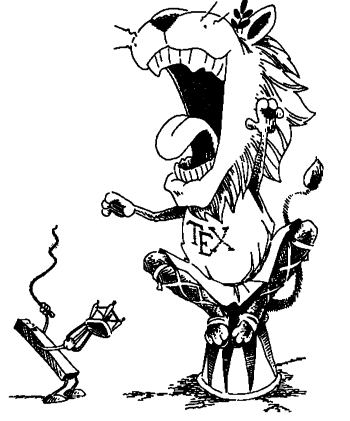
\includegraphics[width = \textwidth]{Chapter3.png}
% 		\caption{\TeX 的控制系列}\label{subfig:1b}
% 	\end{subfigure}
% 	\caption{子图模式测试1:2张图}\label{fig:subfig_test1}
% \end{figure}

% 如\autoref{fig:subfig_test2}是有四张子图的模式,对子图进行交叉引用,如\autoref{subfig:2a}、\autoref{subfig:2b}、\autoref{subfig:2c}和\autoref{subfig:2d}。

% \begin{figure}[htbp]
% 	\centering
% 	\begin{subfigure}[b]{.4\textwidth}
% 		\centering
% 		
\includegraphics[width = \textwidth]{Chapter4.png}
% 		\caption{字体}\label{subfig:2a}
% 	\end{subfigure}
% 	\begin{subfigure}[b]{.4\textwidth}
% 		\centering
% 		
\includegraphics[width = \textwidth]{Chapter5.png}
% 		\caption{编组}\label{subfig:2b}
% 	\end{subfigure}
% 	\begin{subfigure}[b]{.4\textwidth}
% 		\centering
% 		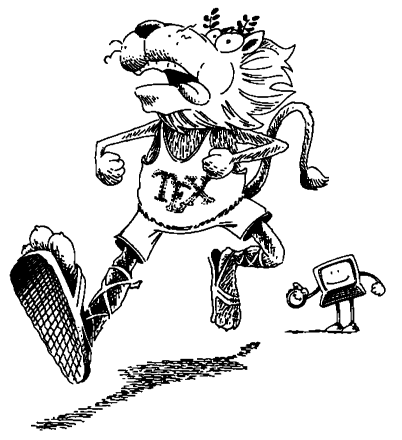
\includegraphics[width = \textwidth]{Chapter6.png}
% 		\caption{运行\TeX}\label{subfig:2c}
% 	\end{subfigure}
% 	\begin{subfigure}[b]{.4\textwidth}
% 		\centering
% 		
\includegraphics[width = \textwidth]{Chapter7.png}
% 		\caption{\TeX 工作原理}\label{subfig:2d}
% 	\end{subfigure}
% 	\caption{子图模式测试2:4张图}\label{fig:subfig_test2}
% \end{figure}

% \subsection{数学模式测试}
% 数学模式测试,主要测试数学字体,编号和交叉引用。这里首先推荐使用\texttt{align}和\texttt{align*}数学模式环境,大多数行间数学模式只需要用这个环境就可以了。

% 交叉引用测试,如交引用命令{\ttfamily \textbackslash eqref}和\texttt{\textbackslash ref}命令的区别。如公式\eqref{eq:test1},公式\ref{eq:test1}显示,\texttt{\textbackslash eqref}命令比\texttt{\textbackslash ref}命令的应用结果多了个括号。

% 如公式\eqref{eq:test3}是单行公式环境,查看公式\eqref{eq:test3}和\eqref{eq:test1}之间的区别,好像在单行公式中没什么区别。
% \begin{align}\label{eq:test3}
% 	f(x) = 2(x + 1)^{2} - 1
% \end{align}

% \texttt{align}公式环境,用在单行中。
% \begin{align}\label{eq:test1}
% 	f(x) = 2(x + 1)^{2} - 1
% \end{align}

% 在这里,中间插入一些文字以形成段落,查看行间公式与上下文之间的间隙。
% \begin{align*}
% 	f(x) = 2(x + 1)^{2} - 1
% \end{align*}
% 在这里,中间插入一些文字以形成段落,查看行间公式与上下文之间的间隙。下一个公式\eqref{eq:test2}是一个公式组,它在“=”位置对齐。
% \begin{align}\label{eq:test2}
% 	f(x) & = 2(x + 1)^{2} - 1\\
% 		 & = 2(x^{2} + 2x +1)-1\\
% 		 & = 2x^{2} + 4x + 1
% \end{align}


% \section{关于引用}
% 图表的引用通过{\ttfamily \textbackslash autoref} 命令即可,使用ST LaTeXTools 插件还能自动补全。如果要修改前缀,那么就用{\ttfamily \textbackslash recnewcommand \textbackslash figureautorefname\{好图\}}即可,详见hyperref宏包说明。

% \section{出现的问题}
% \subsection{\textbackslash texttt}
% 在这里发现一个问题,在下面的例子中可以发现,在中文中使用\textbackslash texttt\{\}命令时,前面的汉字与接下来的英文单词的空隙明显比接下来单词跟汉字的间隙要大,但是其它命令没有什么问题。

% \begin{center}
% \noindent 问题\texttt{问题}问题,问题\textbackslash\texttt{问题}问题。\\
% 问题\texttt{ref} 问题,问题\texttt{\textbackslash ref} 问题。\\
% 问题\textbf{ref}问题,问题\textbf{\textbackslash ref}问题。\\
% 问题\textsf{ref}问题,问题\textsf{\textbackslash ref}问题。\\
% problem \texttt{ref} problem,problem \texttt{\textbackslash ref} problem.\\
% problem \textbf{ref} problem,problem \textbf{\textbackslash ref} problem.\\
% problem \textsf{ref} problem,problem \textsf{\textbackslash ref} problem.
% \end{center}

% 原来的编译环境为texlive 2014,编译环境改为texlive 2015后,问题解决。
